%%5 Development methodology 
\section{Development Methodology}
\label{sec:developmentmethodology}
%What kind of approach are you using to develop your product (e.g. agile, waterfall)? 
%Section 5.1, 5.2

%What are requirements do you use to accept new functionality? 
%Section 5.1, 5.2

%Do you have a definition of done? 
%Client Notes for external defenition. All Must and should haves and other stuff for internal defenition


%Which tools will you be using for your process?
%AWS tools silly

\subsection{Project Methodology}
\subsubsection{Our Findings}
We have conducted research on four popular development methodologies: Agile, Waterfall, Spiral, and Vee. More of our findings and reasoning behind our choices are in the Appendix, however, for brevity, we have include a bulleted list of the pros and cons of each of these methods.


\begin{itemize}
    \item Agile
    \begin{itemize}
        \item Focus on productivity, flexibility, and practicality \cite{manifest}
        \item Lack of documentation and formal studies
    \end{itemize}
    \item Waterfall
    \begin{itemize}
        \item Document driven, simple, clear-cut milestones \cite{spiralmode;}
        \item Inflexible \cite{spiralmode;}
    \end{itemize}
    \item Spiral
    \begin{itemize}
        \item Iterative planning approach for risk-reduction, with continuously increasing detail \cite{spiralmode;}
        \item Heavy-weight, time-consuming
    \end{itemize}
    \item Vee
    \begin{itemize}
        \item Explicit focus on verification and validation; a lot of testing in mind \cite{geeksforgeeks_2023}
        \item Not very little in the way of implementation, and inflexible \cite{spiralmode;} \cite{geeksforgeeks_2023}
    \end{itemize}
\end{itemize}

\subsubsection{Our Methodology of Choice}

All of the aforementioned models have takeaways that we would like to incorporate in our methodology: iterative refinement of requirements of the Spiral Model, the emphasis on verification and validation from the Vee Model, the explicit documentation and demarcation from the Waterfall method, and the flexibility and iterative implementation approach of Agile. Ideally, we'd like all of these aspects from each of the different frameworks, however, we would not be able to get all of them from simply following any one of them verbatim, so we feel the need to engineer our own hybrid approach, that answers Boehm's questions for process methods: "What shall we do next?" and "How long shall we continue to do it?" \cite[p. 61]{spiralmode;}.

\subsubsection{The Chalice Method}



Trying our best to incorporate all of the aspects from the previous methodologies, and what we discussed with industry experts, we came up with the chalice method, which takes inspiration from all of the aforementioned methods and what AWS practitioners actually use. The area under the blue dashed lines is the \textit{Scrum}; this will occur on a regular basis, very similar to a standard Agile method of implementation. This will keep looping until the team is ready to complete the project. The dotted lines represent back-edges that, ideally, should not be followed, but could be if the project calls for it. Stages outside the \textit{Scrum} subsection are complete when a formal document depicting them is complete, much like the Waterfall method. Stages within the \textit{Scrum} subsection are time-based, with a sprint occurring once a week, much like standard Agile, however, alongside the standard completion criteria that come with Agile, the Chalice method adds a condition, namely, the Software check/ review. For our project, we finish at the Operating and Maintenance stage.


\begin{figure}[h]
    \centering
    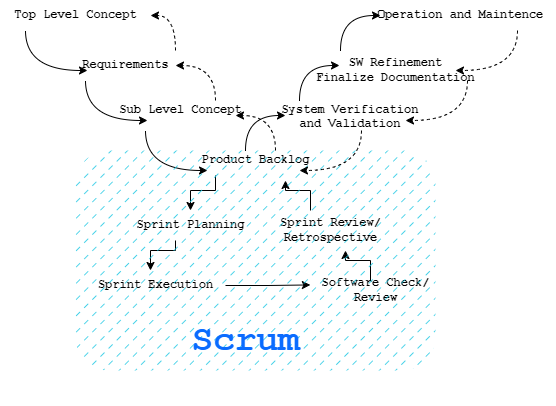
\includegraphics[width=0.7\textwidth]{images/Chalice Method (1).png}
    \caption{The Chalice Method: Alternative to popular methodologies}
    \label{fig:chalice}
\end{figure}

\paragraph*{Top Level Concept (TLC)}
For our project, this part is rather straightforward, it is the grand-scheme concept of what we're building. In this stage, we got introduced to the client, and the project, and selected our low-resource language.

\paragraph*{Requirements}
Similar to the Vee method, this is the stage in which we develop our requirements, and as such, our initial architecture. Based on our highest-level concept, we are able to develop requirements and user stories.

\paragraph*{Sub-Level Concept (SLC)}
Using the requirements, the team is able to come up with a more detailed architecture, which for this project, will give us a solid, detailed foundation and help us select and pinpoint which AWS services we'd really like to use and focus on. Furthermore in this stage, we'd solidify our requirements and technologies, which would lead to a very straightforward implementation approach, since, ideally, all of the architectural kinks should be ironed out during this stage.

\paragraph*{Product Backlog}
This is the first and last stage of the \textit{Scrum} subsection of the model. This replaces the "Implementation" step of the Vee model, giving the team a more rigid framework to actually implement and create the software, based on Agile. Unlike the Vee model, this model is not entirely dependent on previous documentation and different levels of conceptualization to implement the product, instead, this model allows the different concepts to pave the way for the engineers, and create structure, while still allowing them to move freely and make changes within their sprints. This stage has the team examining the product backlog, creating, modifying, and removing user stories and requirements ad-hoc, but at fixed points in the cycle.

\paragraph*{Sprint Planning and Sprint Execution}
These steps are identical to the normal Scrum methodology, wherein our Sprint Plannings are to occur once a week, and our execution is to take place by daily stand-up.

\paragraph*{Software Check/Review}



Based on the conversations we have had with industry experts, we believe, within the Agile-inspired subsection of the Chalice Method, we needed a mechanism specifically designed for receiving feedback and creating documentation, which is where Agile falls short. Our solution to this problem was to modify code reviews frequently found in Agile by also placing emphasis on documentation and code clarity. We perform these modified code reviews at the end of a sprint. Software that meets requirements \textbf{must} pass this step before being complete.


%%

 %In this stage, engineers are put in groups, or partnerships, where they are to briefly examine each others' work, and ensure that other engineers can quickly identify the purpose and the interfaces of their work, and the contributing engineer can quickly justify it with respect to the rest of the system. Ideally, this stage should occur quickly, over the span of about an hour, having everything well documented beforehand, however, if this is not the case, now is the time to fix it. The most significant part of checking the quality of our work is by making sure the translations of the blog posts are accurate. This will be ensured in our weekly meetings with domain experts so that they can assess the quality of the translation and we can improve our service upon this consultation.

%
%
%


\paragraph*{System Verification and Validation}
After a sufficient number of sprints have been completed, the project can move onto the right wall of the chalice, which begins, similar to the Vee method, with the System Verification and Validation stage, where the team ensures that the system as whole works, using various testing methods, and that it meets the requirements.

\paragraph*{SW Refinement and Finalize Documentation}
In this stage, the team ensures that the software is organized and finalizes formal as well as in-line documentation to prepare for the hand-off. If SW refinement occurs, the team may need to take a step back to the previous step.

\paragraph*{Societal Relevance and Ethical Approach}
sIt is not designated in the diagram, however, during the development process of our translation service, we will critically think about the impacts our application could have on society, especially on Native Turkish Speakers. The possible concerns which may arise due to the quality of the application will be kept in mind throughout the development process, and the ethical side of our application will be thought out to make sure we follow the best practices without any negative affect on society. 

\subsection{Communication \& Tools}

As a team, we decided that we will use mainly 3 channels of communication, Discord for online meetings, WhatsApp for general communication, and Mattermost for communication with TAs and the course staff. We use Discord for general meetings related to the project and our daily stand-up sessions where each one of us briefs the entire team on what we, as individuals, have been working on the previous day, what we hope to achieve in the future and ask for clarification or give useful information related to the project and our schedule throughout the meeting. We also have a shared Google Calendar that helps keep us on the same page with regard to the schedule as it is easier than coordinating meetings/deadlines over text communication since it is easy to forget or miss a message. We are also interested in meeting in person, either at AWS’ offices or on campus as we find that we work best as a group when we are all in the same location but we are not sure if working at AWS offices is feasible yet. Furthermore, we use AWS’ internal service, Amazon Chime, to have online meetings with AWS employees. We meet with the technical team at AWS every week on Fridays to discuss our progress and to ask any questions we might have. Furthermore, we will have Gitlab's scrumboard to keep track of our issues as we go .

